\section{Javascript}

	\subsection{requestAnimationFrame();}

Für einige Operationen in JavaScript \footcite[vgl.][]{reflow} muss ein Reflow durchgeführt werden, mit dem die Positionen der Elemente der Website neu berechnet werden. Zwangsläufig muss danach auch ein Repaint durchgeführt werden, damit mögliche Änderungen auf dem Bildschirm sichtbar werden. Dies geschieht unabhängig von den standardmäßigen 60 Repaints pro Sekunde, wodurch mehr als 60 Repaints pro Sekunde enstehen, was die FPS Zahl künstlich auf über 60 angehebt. Manche Endgeräte können eine solche Last nicht tragen, es kommt zu Lags, erhöhtem Stromverbrauch (vor allem bei mobilen Endgeräten von Relevanz), folglich bleibt dem Nutzer nur noch das Verlassen der Seite übrig. Hier setzt \lstinline{requestAnimationFrame()} an.
Die \lstinline{requestAnimationFrame}-Funktion synchronisiert den Aufruf einer übergebenen Callback-Funktion mit dem Repaint des Browsers, sodass die Website erst dann neu gerendert wird, wenn alle notwendigen Berechnungen und Reflows abgeschlossen sind.


\subsection{Animation Core}
Um Animationen auf einer Website zu realisieren, kann man auf Frameworks wie jQuery zurückgreifen. Jedoch benutzen die meisten Frameworks intervallgesteuerte Animationsbibliotheken, die den Vorteil von \lstinline{requestAnimationFrame} nicht ausnutzen können. Deshalb wird im Folgenden ein auf Rekursion basiertes Animationsframework für Smooth Scrolling entwickelt, das später bei der Umsetzung unterschiedlicher Navigationsmöglichkeiten von Bedeutung sein wird, orientiert an \footcite[vgl.][]{rAF}.

\begin{lstlisting}[caption=Die Funktionen setScLPos und getScLPos., label=js_get_set]
function getScLPos() {
	if (self.pageXOffset) return self.pageXOffset;
	if (document.documentElement && document.documentElement.scrollLeft)
		return document.documentElement.scrollLeft; 
	if (document.body.scrollLeft) return document.body.scrollLeft;
		return 0; 
}
function setScLPos(pos) {
	if (document.documentElement.scrollLeft || document.documentElement.scrollLeft == 0)
		document.documentElement.scrollLeft = pos;
	if (document.body.scrollLeft || document.body.scrollLeft == 0)
		document.body.scrollLeft = pos;
}
\end{lstlisting}

Um Browserübergreifend zu funktionieren, muss das Framework zunächst über Funktionen zum Setzen und Abfragen der Scrollposition verfügen (siehe Codeauszug \ref{js_get_set}). In der \lstinline{getScLPos}-Funktion werden dabei zunächst die verschiedenen Variablen abgefragt, die die Scrollposition enthalten. Dabei ist darauf zu achten, dass die If-Bedingung die Werte 0, \lstinline{undefined} und \lstinline{null} als \lstinline{false} interpretiert, weshalb davon auszugehen ist, dass die If-Bedingung auch dann übersprungen wird, wenn die jeweilige Variable gleich 0 ist. Deshalb wird am Ende der Funktion 0 ausgegeben. Im Gegensatz dazu muss in der \lstinline{setScL} Funktion, mit der die Scrollposition gesetzt wird, explizit geprüft werden, ob die Variable existiert, indem die Gleichheit auf 0 auch geprüft wird. Erst dann kann entschieden werden, welche Variable in ihrem Wert geändert wird.

\begin{lstlisting}[caption=Globale Variablen des Animationsframework., label=js_globals]
var startX = null;
var startY = getScLPos();
var dest = 0;
var duration = 1000;
var reqID = 0;
\end{lstlisting}


Leider können der Callback Funktion als Argument der requestAnimationFrame-Funktion keine Parameter übergeben werden, weshalb hier die Parameter als globale Variablen deklariert werden (siehe Codeauszug \ref{js_globals}). Bei diesen Parametern handelt es sich um den Startzeitpunkt (\lstinline{startX}, weil Zeit meistens auf X-Achse), den Startwert (\lstinline{startY}), die Dauer der Animation (\lstinline{duration}) und den Endwert (\lstinline{dest} wie destination). Mit diesen Parametern kann zu jedem Zeitpunkt der Animation der jeweilige Wert explizit durch Interpolation berechnet werden. Die Variable \lstinline{reqID} speichert IDs von ausstehenden \lstinline{requestAnimationFrame()}-Aufrufen, welche mit Hilfe der ID abgebrochen werden sollten, bevor neue Aufrufe ausgelöst werden, da auf Grund der begrenzten Zeit innerhalb eines AnimationFrames nur eine begrenzte Anzahl an Operationen durchgeführt werden kann. Das Stapeln von \lstinline{requestAnimationFrame()}-Aufrufen ist zudem deshalb unsinnig, da in diesem Beispiel eine Funktion mehrmals durchlaufen wird, wobei alle relevanten Variablen, die die Funktion verändert, vom nächsten Funktionaufruf wieder verändert werden. Hier ist also nur der aktuelle Funktionsaufruf von Bedeutung. Außerdem stellt das parallele Ausführen von Animationen ein Problem dar, da auf die globale Variable der Scrollposition zugegriffen wird. Bevor eine neue Animation gestartet wird, muss die alte Animation beendet werden, da es sonst zur Inkonsistenz der globalen Scrollpositionsvariable kommt, wodurch Bugs auftreten. Dabei reicht es aus, einen Rekursionsschritt abzubrechen, um die ganze Rekursion zu beenden.

\begin{lstlisting}[caption=Die Funktion cancelAnim., label=js_cancelanim]
function cancelAnim() {
	if (reqID) {
		cancelAnimationFrame(reqID);
		reqID = 0;
	}
}
\end{lstlisting}

\lstinline{requestAnimationFrame()} liefert als Rückgabewert eine ID, die solange gültig ist, wie der Request noch aussteht. Speichert man diesen Wert in \lstinline{reqID}, bedeutet das, dass \lstinline{requestAnimationFrame()} bereits aufgerufen, aber noch nicht vom Browser abgearbeitet worden ist, wenn \lstinline{reqID} einen Wert verschieden von 0 hat. In diesem Falle muss die Anfrage mittels \lstinline{cancelAnimationFrame()} und jener ID abgebrochen werden (wie in Codeauszug \ref{js_cancelanim}). Danach wird \lstinline{reqID} auf 0 gesetzt, womit nun neue AnimationFrames angefragt werden dürfen.

\begin{lstlisting}[caption=Die Funktion scAnim., label=js_scanim]
function scAnimate() {
	cancelAnim();
	reqID = requestAnimationFrame(scStep);
}
\end{lstlisting}

Die Funktion \lstinline{scAnimate} (Codeauszug \ref{js_scanim}) ist für den Start der Rekursionsschleife zuständig. Nach Abbruch aller Animationen wird unter Speicherung der ID ein neuer \lstinline{requestAnimationFrame()}-Aufruf gestartet, mit dem die Rekursionsschleife der Funktion \lstinline{scStep} betreten wird.

\begin{lstlisting}[caption=Die Funktion scStep., label=js_scstep]
function scStep(timestamp) {
	if (startX == null)
		startX = timestamp;
	var passed = timestamp - startX;
	var progress = passed / duration;
	var value = startY + ((dest - startY) * delta(progress));
	setScLPos(value);
	if (progress < 1)
		reqID = requestAnimationFrame(scStep);
	if (progress >= 1) {
		startX = null;
		startY = getScLPos();
	}
}
\end{lstlisting}

Diese Funktion scStep\footcite[vgl.][]{rAF} (Codeauszug \ref{js_scstep}) bildet das einzelne Rekursionsglied. Zunächst wird geprüft, ob \lstinline{startX} null ist, da dies bedeutet, dass die Animation noch nicht begonnen hat. Ist dies der Fall, wird \lstinline{startX} auf die aktuelle Zeit gesetzt, die von \lstinline{requestAnimationFrame} bei der Ausführung übergeben wird. Nun hat \lstinline{startX} einen Wert, der innerhalb der Animation nicht mehr verändert wird. Auf Grund der vergangenen Zeit (Differenz zwischen aktuellem Timestamp und Startzeit) und der bereits bestimmten Dauer der Animation kann der Fortschritt der Animation berechnet werden, der sich zwischen 0 und 1 bewegen sollte. Aufgrund der nicht vorhersehbaren Verzögerung beim Aufruf des Rekursionsschrittes durch requestAnimationFrame kann die Variable Progress auch Werte größer als 1 enthalten. Im Allgemeinen lässt sich jedoch sagen, dass die Animation bei Werten größer 1 zu Ende ist. Dann wird das oben angesprochene \lstinline{startX} wieder auf null zurückgesetzt und \lstinline{startY} wird aktualisiert. Ist die Animation noch nicht beendet, ruft sich \lstinline{scStep} für den nächsten Frame erneut auf.

In jedem Schritt der Animation wird in value der interpolierte Wert für die Scrollposition übernommen. Den Verlauf dieser Werte regelt die Funktion \lstinline{delta()} (Codeauszug \ref{js_delta}), hier entspricht der Verlauf einer kubischen easeOut-Funktion \footcite[vgl.][]{easeOut}.



\begin{lstlisting}[caption=Die Funktion delta., label=js_delta]
function delta(prog) {
	return 1 - Math.pow(1 - prog, 3);
}
\end{lstlisting}

Nun ist das Animationsframework für die Zwecke der Digital-Home-Seite einsatzfähig.

\subsection{Parallax Funktion}
Die Startseite wirkte beim Scrollen bisher durch das minimalistisch flache Design sehr statisch und platt. Um der Seite trotzdem Tiefe und 3-Dimensionalität zu geben, wurde ein Parallax-Scrolling-Effekt für das Titelbild jeder Seite implementiert.

\begin{lstlisting}[caption=Das Onscroll-Event und die Parallax-Callbackfunktion., label=js_scrollex]
function prllx() {
	var curr_x = getScLPos();
	var speed = 0.5;
	p1_img.style.left = curr_x * speed + 50 + "px";
	scroll_correct = false;
}
var scroll_correct = false;
function scrollex() {
	if (scroll_correct == false) {
		scroll_correct = true;
		requestAnimationFrame(prllx);
	}
}
window.onscroll = scrollex;
\end{lstlisting}

Im Codeauszug \ref{js_scrollex} sieht man die Zuweisung der Funktion \lstinline{scrollex()} zum Onscroll-Eventhandler. Da das Scrollevent vor allem auf Touchpads mehrere Male pro Sekunde aktiviert wird, muss sichergestellt sein, dass nicht mehrere Events pro Frame mehrere Funktionsaufrufe pro Frame auslösen. Dafür wird die Variable \lstinline{scroll_correct} eingeführt. Sie ist standardmäßig false und wird auf true gesetzt sobald ein Scrollevent einen Funktionsaufruf der Parallaxfunktion \lstinline{prllx()} auslöst, danach kann diese Funktion, die für die parallaxe Verschiebung des Titelbildes verantwortlich ist, nicht mehr aufgerufen werden bis sie zum nächsten AnimationFrame ausgeführt wird. Zum Ende der Funktion wird \lstinline{scroll_correct} auf false zurückgesetzt, damit sie beim nächsten Scrollevent wieder aufgerufen werden kann. Innerhalb der Funktion \lstinline{prllx()} wird die Verschiebung des Bildes abhängig von der aktuellen Scrollposition ausgerechnet. Ist die Position konstant, so scrollt das Bild mit dem Content und der Effekt entspricht einer absoluten Positionierung mit CSS. Ist die Position des Bildes gleich der Scrollposition, so bewegt sich das Bild mit dem Viewport, was fixierter Positionierung mit CSS entspräche. In diesem Beispiel wurde der Faktor 0.5 (Variable speed) gewählt, womit sich das Bild halb so schnell wie der Content in Scrollrichtung bewegt. Dadurch entsteht der gewünschte 3D-Effekt.




\subsection{Canvas}
\label{descr_canvas}

Da sich Teile der Website noch im Bau befinden, müssen Platzhalter für diese Seiten her. Einfache Textseiten wie `hier wird gebaut` würden langweilig wirken und die geringe Wertschätzung der Seite von Seiten der Entwickler und Designer zeigen. Deshalb muss man sich für Error- und Baustellenseiten etwas besonderes einfallen lassen, um die Seite mit Inhalt zu füllen und dem User als Kunden etwas zu bieten, was er in guter Erinnerung behalten kann. Im Bezug auf Kapitel \ref{emo_col} wurde eine Seite entwickelt, die auf der einen Seite mit Hilfe des Farbschemas Emotionen hervorrufen kann und gleichzeitig den Satz `hier wird gebaut` verbildlicht. Dafür wurde eine parallax scrollende Seite entwickelt, auf der die Skyline einer Stadt zu sehen ist mit wechselndem Himmel, der den Verlauf des Tages darstellen soll. In der Skyline lassen sich Kräne, Helikopter und Baustellen erkennen, die sich auf die Baustellenseite beziehen. Außerdem soll die Stadt technologischen Fortschritt verdeutlichen, den Digital Home verkörpern will.
\begin{figure} [h]
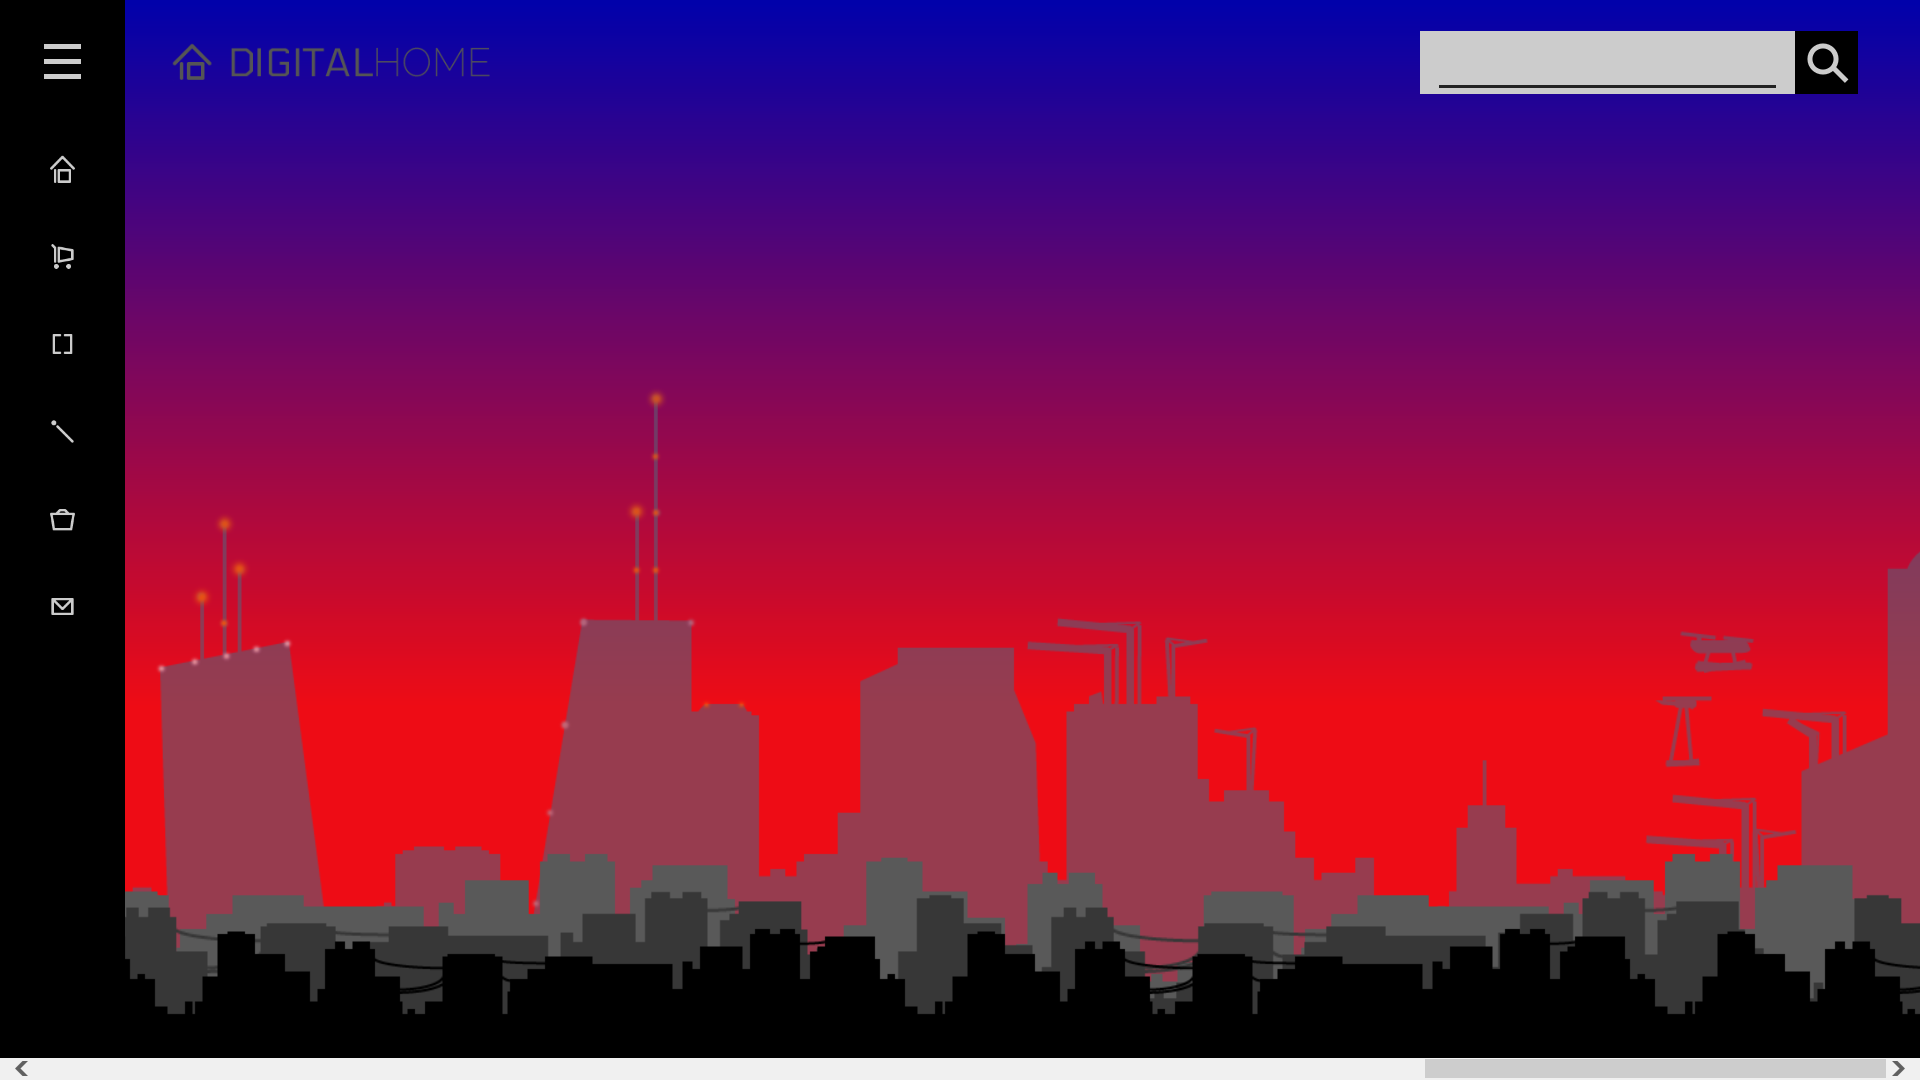
\includegraphics[width=\textwidth]{./img/js_canvas_highlight.png}
\caption{Der Höhepunkt der Canvas-Animation}
\label{js_canvas_highlight}
\end{figure}
Der Höhepunkt der Hintergrundanimation tritt nach ca. 13 Sekunden auf, wenn sich der Himmel orientiert an dem Farbschema der Seite blau orange färbt, und ist in Abbildung \ref{js_canvas_highlight} zu sehen.

Besonders interessant ist hier die Animation des Farbverlaufes mit Hilfe von Arrays. Für jeden Farbstop des Farbverlaufes gibt es drei Farbvektoren je in Form eines Arrays mit drei Elementen. Der erste (\lstinline{rgb}) speichert den aktuellen RGB-Wert des Farbstops. Der zweite (\lstinline{min}) speichert die Anfangswerte der drei Komponenten zum Beginn eines Intervalls. Im Gegenzug speichert \lstinline{max} die Endwerte der Komponenten. Dadurch kann mit \lstinline{min} und \lstinline{max} die aktuelle Farbe interpoliert werden, wie in Codeauszug \ref{js_interpol} zu sehen. Die Zusätze \lstinline{t} und \lstinline{b} stehen für \lstinline{top} und \lstinline{bottom} und signalisieren die Zugehörigkeit der Vektoren zum oberen bzw. unteren Farbstop.

\begin{lstlisting}[caption=Jede Komponente des Farbvektors wird einzeln interpoliert., label=js_interpol]
for (var i = 0; i < 3; i++) {
	var mt = (maxt[i] - mint[i]) / ((etim - stim));
	var mb = (maxb[i] - minb[i]) / ((etim - stim));
            
	rgbt[i] = mint[i] + mt * (time * 24 / dayLength - stim);
	rgbb[i] = minb[i] + mb * (time * 24 / dayLength - stim);

	rgbt[i] = rgbt[i] >= 0 ? rgbt[i] : 0;
	rgbb[i] = rgbb[i] >= 0 ? rgbb[i] : 0;

	rgbt[i] = rgbt[i] <= 255 ? rgbt[i] : 255;
	rgbb[i] = rgbb[i] <= 255 ? rgbb[i] : 255;

	colt += ('0' + (rgbt[i] | 0).toString(16)).substr(-2);
	colb += ('0' + (rgbb[i] | 0).toString(16)).substr(-2);         
}
\end{lstlisting} 

 \begin{lstlisting}[caption=Die Funktion daytime wird in jedem Animationsframe einmal aufgerufen., label=js_daytime]
var stim = 0;
var etim = 0;
var time = 50;
       
function daytime() {
	dayLength = 240;
	time = (time + 1) % dayLength;
	colt = '#';
	colb = '#';

	if (time < dayLength * 6 / 24 && tswitch != 0) {
		tswitch = 0;
		stim = 0;
		etim = 6;
		mint = [0, 0, 50];
		minb = [50, 0, 50];
		maxt = [82, 1, 187];
		maxb = [207, 84, 70];
	} else if ...
	...
}
\end{lstlisting} 

Um verschiedene Tageszeiten interpolieren zu können, müssen sich die Anfangs und Endwerte der Farben abhängig von der Tageszeit ändern. Dazu werden die Variablen \lstinline{stim} für die Startzeit und \lstinline{etim} für die Endzeit eingeführt, die Werte zwischen 0 und 24 besitzen. Sie zeigen, in welchem Interval des Tages (in Stunden) sich die Animation gerade befindet. Die Variable \lstinline{time} stellt den Einzelschritt in der Animation dar und wird daher hochgezählt. Einen Ausschnitt des Codes, der das Interval zwischen 0Uhr und 6Uhr definiert, sieht man in Codeauszug \ref{js_daytime}.

\subsection{Menü}
Läuft auf dem Client-PC kein Javascript, so muss das Menü trotzdem zugänglich sein. Deswegen ist das Menü grundsätzlich offen und wird erst durch ein funktionierendes Javascript beim Laden der Seite geschlossen, wie in Codeauszug \ref{js_menuevent} zu sehen.

 \begin{lstlisting}[caption=Die Funktion tog\_m() öffnet bzw. schließt das Menü., label=js_menuevent]
window.onload = tog_m;
var tog_menu = 1;
document.getElementById("m_button").addEventListener("click", tog_m);

function tog_m() {
	if (tog_menu == 0) {
		document.getElementById("navi").className = "active";
		document.getElementById("mb1").className = "mact";
		document.getElementById("mb2").className = "mact";
		document.getElementById("mb3").className = "mact";
		tog_menu = 1;
	} else {
		document.getElementById("navi").className = "idle";
		document.getElementById("mb1").className = "mnorm";
		document.getElementById("mb2").className = "mnorm";
		document.getElementById("mb3").className = "mnorm";
		tog_menu = 0;
	}
}
\end{lstlisting} 

\subsection{Navigation innerhalb der Seite}
Damit ein Nutzer auf die Informationen einer Website zugreifen kann, muss die Navigation hin zu der Seite, aber auch innerhalb der Seite entsprechend ausgeführt werden. Dabei müssen auch unterschiedliche Nutzerverhalten berücksichtigt werden. Dieser Abschnitt wird sich vor allem um die Navigation innerhalb der Seite drehen. Es werden die Vor- und Nachteile unterschiedlicher Methoden angesprochen, danach wird abgewägt, ob deren Implementierung sinnvoll ist oder nicht.
Die Maßnahmen treffen vor allem Desktopnutzer, da Touchscreennutzer mit der Navigation keine Probleme haben sollten.
\subsubsection{Maus}
Die wohl am weitesten verbreitete Methode der Interaktion mit einer Seite ist die Maus bzw. das Touchpad. Viele Nutzer können jedoch mit der Maus nicht seitwärts scrollen. Schaut man sich auf anderen Seiten mit horizontalem Scrolling (z.B. die Website von Stephane Tartelin
\footcite[zu finden auf:][]{tartelin} oder das windows 8 startmenü) um, dann ist auf den meisten Websites eine Übersetzung von vertikalem in horizontales Scrolling implementiert. Es kann also davon ausgegangen werden, dass Nutzer auf einer horizontal scrollenden Seite daran gewöhnt sind, mit ihrem Mausrad zu arbeiten. Deshalb ist es notwendig, eine Übersetzung von vertikalen Mausradbewegungen in horizontales Scrolling zu implementieren. 
	
 \begin{lstlisting}[caption=Die unterschiedlichen Eventhandler des Mausrads., label=js_mousehandler]
window.addEventListener("wheel", mousewheel, false);          //non FF
window.addEventListener("DOMMouseScroll", mousewheel, false); //FF
window.onmousewheel = mousewheel;
\end{lstlisting} 

Den drei Mausradeventhandlern  \footcite[vgl.][]{jsMousewheel} (siehe Codeauszug \ref{js_mousehandler}) wird eine Funktion als Callback übergeben, mousewheel(). Dies ist zu sehen in Codeauszug \ref{js_mousewheel}. Diese Funktion bekommt das Event e als Übergabeparameter. Dabei ist jedoch darauf zu achten, dass die Eigenschaft, die die Bewegung des Mausrads speichert bei unterschiedlichen Events in unterschiedlichen Browsern unterschiedliche Namen hat. So betrifft e.wheelDelta Chrome und Internet Explorer, während e.detail von anderen Browsern benutzt wird. Speziell in Chrome kann sogar wheelDeltaY abgerufen werden, was einem nur die vertikale Komponente der Drehung des Mausrads liefert. Interessant, da Touchpads auch Mousewheelevents aktivieren. Die meisten Touchpads haben im Treiber bereits Smoothscrolling integriert, Mäuse nicht. Ein Javascript basiertes Smoothscrolling mit dem bereits entwickelten Animationsframework würde mit dem Smoothscrolling von Touchpads interferieren, soll aber gleichzeitig für das horizontale Scrolling mit Mausrädern eingesetzt werden, um eine bessere User-Experience zu gewährleisten. In Chrome kann man dies trennen. Das Mausradscrolling wird hier in horizontales übersetzt und mit Smoothscrolling verschönert. In den anderen Browsern muss leider ein Kompromiss her, denn Smoothscrolling würde auf Touchpads nicht funktionieren und ohne Scrollübersetzung könnten Mausnutzer nur schwer auf der Seite navigieren. Deshalb wird hier abhängig von der Mausradbewegung die Scrollposition der Seite ohne Animation aktualisiert, wodurch das Smoothscrolling der Touchpads funktionsfähig bleibt und Mausnutzer trotzdem navigieren können, wenn auch mit Einbußen in Sachen User-Experience.

 \begin{lstlisting}[caption=Die Funktion mousewheel() regelt die Verarbeitung des Mausraddelta., label=js_mousewheel]
function mousewheel(e) {
	var e = window.event || e;
	if (e.wheelDeltaY) {
		//Webkit
		var delta = e.wheelDeltaY / 40;
		startX = null;
		startY = getScLPos();
		dest = startY - delta * document.documentElement.clientWidth * 0.13;
		duration = 500;
		scAnimate();
	} else if (e.wheelDelta) {
		//IE
		cancelAnim();
		var delta = e.wheelDelta / 40;
		setScLPos(getScLPos() - delta * 20);
	} else {
		//Others
		cancelAnim();
		var delta = -e.detail;
		setScLPos(getScLPos() - delta * 20);
	}
}
\end{lstlisting} 

\subsubsection{Pfeiltasten}
Eine weitere Alternative zum Scrolling ist die Verwendung von Pfeiltasten. Sie funktioniert auf allen Endgeräten mit Tastatur. Da das normale Scrolling mit Pfeiltasten sehr langsam ist, soll es durch Smoothscrolling ersetzt werden. Dabei bedient man sich des Tastendruck-Eventhandlers onkeydown. Er übergibt der Callback Funktion die Eventeigenschaften, darunter der Keycode, der das ASCII-Zeichen der gedrückten Taste enthält. Die Keycodes 37 und 38 repräsentieren die Pfeile nach links und nach oben, während 39 und 40 die Pfeile nach rechts und nach unten repräsentiert. Davon abhängig werden die globalen Animationsvariablen gesetzt und das Animationsframework übernimmt den Rest. \lstinline{e.preventDefault()} unterbindet das Standardverhalten des Browsers unter dem jeweiligen Event.

 \begin{lstlisting}[caption=Abfangen des Tastendrücken durch das onkeydown-Event, label=js_mousewheel]
window.onkeydown = function (e) {
	if (e.keyCode == 37 || e.keyCode == 38) {
		startX = null;
		startY = getScLPos();
		dest = startY - document.documentElement.clientWidth * 0.4;
		duration = 1000;
		scAnimate();
		e.preventDefault();
	} else if (e.keyCode == 39 || e.keyCode == 40) {
		startX = null;
		startY = getScLPos();
		dest = startY + document.documentElement.clientWidth * 0.4;
		duration = 1000;
		scAnimate();
		e.preventDefault();
	}
}
\end{lstlisting} 
